\chapter{Wstęp}
\label{cha:wstęp}
Morfologia krwi (ang. \textit{complete blood count}) jest jednym z~najczęściej przeprowadzanych badań. Dostarcza ona informację o~komórkach krwi pacjenta, w~tym liczbę komórek każdego typu krwinek i~wartość stężenia hemoglobiny. Zgodnie z~zaleceniami powinno się wykonywać je przynajmniej raz do~roku w~celach profilaktycznych. Jest to~też jedno z~pierwszych badań stosowanych w~diagnostyce schorzeń. Według reportu GUS 42\% osób decydujących się na~badanie labolatoryjne wybiera właśnie badanie krwi (Rys. \ref{GUS_Zdrowie2016}) \cite{GUS_Zdrowie2016}.

\begin{figure}[h]
\begin{center}
	\begin{tikzpicture}[scale = 0.8]
		\pie [polar, explode=0.1, text=legend] 
    		{42/badania krwi,
     	36/badania moczu,
     	9/cytologia, 
     	2/PSA, 
     	11/inne}
	\end{tikzpicture}
\end{center}
\caption{Typy wykonanych badań labolatoryjnych na~podstawie \cite{GUS_Zdrowie2016}.}
\label{GUS_Zdrowie2016}
\end{figure}

{\parindent0pt % disables indentation for all the text between { and }
Biorąc pod~uwagę stan ludności i~ograniczoną liczbę personelu medycznego w~szpitalach manualne wykonywanie tego typu badań jest problematyczne i~zajmuje dużo czasu. Poprzez usunięcie czynnika ludzkiego można uzyskać większą poprawność i~zwiększyć poduktywność personelu medycznego. \textbf{Celem pracy jest zbudowanie narzędzia do~automatycznej klasyfikacji białych krwinek opartego na~głębokich konwolucyjnych sieciach neuronowych. Oczekiwanym wynikiem pracy jest zbudowanie sieci neuronowej określającej z~jak najlepszą doładnośćią jaki typ krwinki znajduje się na~zdjęciu, a~następnie modyfikacja zarówno parametrów sieci jak i~danych wejściowych w~celu zbadania wpływu zmian na~działanie modelu.} na~wejściu do~sieci wprowadzane są~zdjęcia pojedynczych krwinek, wykonane pod~mikroskopem. W~tym celu została wykorzystana baza danych na~licencji MIT, zawierająca cztery klasy krwinek najliczniej występujące w~składzie krwi. Każde zdjęcie jest oryginalnie przyporządkowane do~odpowiedniej klasy, zgodnie z~widniejącym na~nim elementem morfologicznym \cite{kaggle_database}.

Przed użyciem bazę podzielono na~rozłączne zbiory: uczący, walidacyjny i~testowy. za~pomocą zbiorów uczącego i~walidacyjnego wyuczono i~dostrojono klasyfikator. Dzięki danym ze~zbioru testowego, zawierającego zdjęcia nigdy nie~wprowadzane na~wejście sieci, sprawdzono skuteczność zastosowanej metody.

Program został napisany w~języku Python, który jest dobrze przystosowany do~przetwarzania, analizy i~modelowania danych. do~implementacji sieci użyta została biblioteka Keras, która jest wysokopoziomowym API biblioteki TensorFlow.
}
%---------------------------------------------------------------------------
\section{Motywacja pracy}
\label{sec:motywacja_pracy}
Morfologia krwi to~podstawowe badanie wykonywane w~celu diagnostyki lub~profilaktyki. Analizuje ono cechy i~liczebność zarówno krwinek czerwonych, które stanowią ok.40\% objętości krwi, jak i~białych, stanowiących ok. 0,1\% objętości krwi \cite{krwiodawcy_sklad_krwi}. Wyniki badania krwinek białych mogą dać informację o~zakażenu wirusowym, bakteryjnym lub~pasożytniczym organizmu \cite{morfologia_krwi_wyniki_interpretacja}. Ocena parametrów tego typu krwinek jest też pomocna w~diagnostyce stanu immunologicznego, białaczki i~chorób rozrostowych. Zwiększenie sumarycznej liczby leukocytów do~ok. 20 000 świadczy o~zakażeniu organizmu. Podwyższona liczba neutrofili oznacza ostre zakażenie bakteryjne lub~stan po~urazie z~masywnym krwotokiem. w~przypadku gdy pacjent cierpi na~alergię lub~jest zakażony pasożytami w~organiźmie będzie za~dużo eozynofili. Skutkiem zakażenia wirusowego i~przewlekłych infekcji bakteryjnych jest wyższy poziom limfocytów. Wzrost liczby monocytów świadczy o~chorobie zapalnej, a~ich spadek o~zaburzeniu odporności \cite{morfologia_krwi_wyniki_interpretacja}.

{\parindent0pt % disables indentation for all the text between { and }
Znaczenie diagnostyczne mają bezwzględne liczby poszczególnych rodzajów krwinek białych, zawartych we krwi obwodowej \cite{diagnostyka_laboratoryjna}. Obecnie proces ten jest wykonywany manualnie za~pomocą hemocymetru (Rys. \ref{blood_cells_microscope}) lub~automatycznie z~użyciem np. technologii VCS, pomiarem impedancji czy~pomiarami z~użyciem lasera. Precyzyjne pomiary liczby poszczególnych rodzajów krwinek białych możliwe są~jedynie dzięki metodom automatycznym, przy pomocy analizatorów hematologicznych \cite{diagnostyka_laboratoryjna}.

\begin{figure}[h]
	\centering
		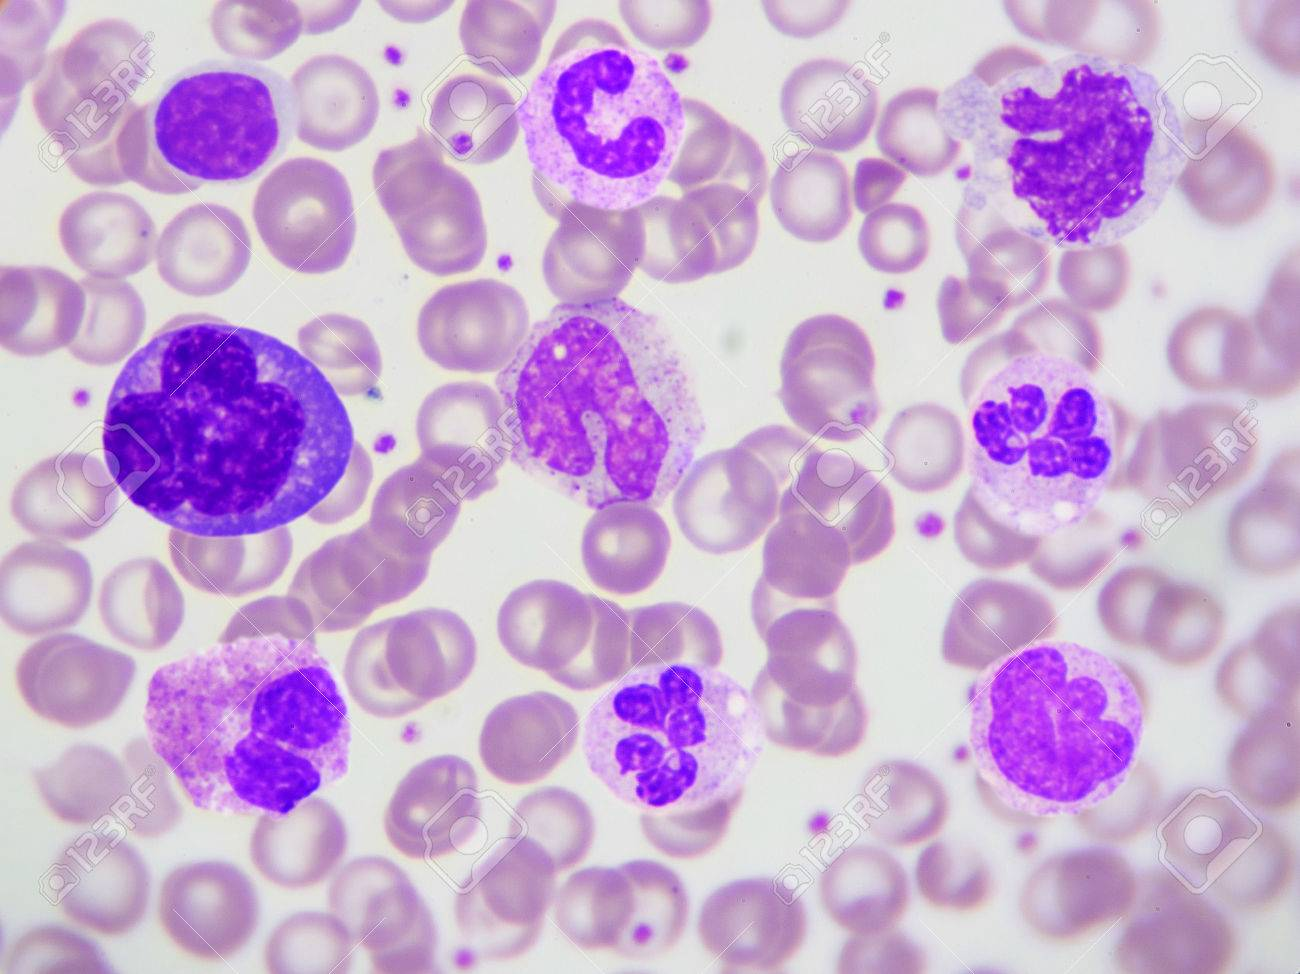
\includegraphics[scale=0.6]{blood_cells_microscope}
	\caption{Widok krwinek badanych pod~mikroskopem \cite{cells_microscope}.}
	\label{blood_cells_microscope}
\end{figure}


Ciekawą alternatywą dla tych metod byłoby zastosowanie automatycznego zliczania komórek opartego na~klasyfikacji przynależności do~danego typu na~podstawie analizy obrazów przez~sieć neuronową. Byłaby to~metoda nie~wymagająca ingerencji czynnika ludzkiego, jak to~ma miejsce w~przypadku badania manualnego, a~jednocześnie tańsza niż stosowane pomiary automatyczne. Zmniejszenie liczby ręcznych procesów i~nadmiaru próbek podczas rutynowych badań zwolniłoby miejsce dla innych ważnych zadań, zwiększyło wydajność i~poprawiło jakość analiz. w~pełni zautomatyzowany proces zmniejszyłby indywidualne ryzyko błędów.

Bazę do~zbudowania takiego narzędzia stanwiłaby sieć rozpoznająca typ krwinki na~zdjęciu i~właśnie tą~częścią zajmuje się niniejszy projekt. w~pracy zdecydowano się na~sieć konwolucyjną głęboko uczoną i~w zależności od~parametrów zbadano precyzyjność jej działania. w~tym celu przetestowano wiele kombinacji doboru składowych modelu, a~poniżej opisano kilka najciekawszych przypadków.
}
%---------------------------------------------------------------------------
\section{Cel i~zrealizowane zadania}
\label{sec:cel_i_zrealizowane_zadania}

Aby zbudować narzędzie do~klasyfikacji krwinek białych najpierw przeprowadzono analizę przydatności takiego rozwiązania na~rynku oraz sprawdzono jakie metody są~obecnie wykorzystywane w~ badaniach krwi. Analiza wykazała zasadność stworzenia tego typu automatyzacji.

{\parindent0pt % disables indentation for all the text between { and }
W celu zrealizowania pracy inżynierskiej wykonano następujące zadania:
}
\begin{itemize}
\item analiza problemu badawczego, zapoznanie się z~zagadnieniem badań morfologicznych,
\item zapoznanie się z~obecnym stanem wiedzy na~temat sieci neuronowych głęboko uczonych oraz sieci konwolucyjnych i~przegląd dostępnych rozwiązań podobnych problemów w~lieraturze,
\item wybór bazy danych i~zapoznanie się z~jej zawartością,
\item zaplanowanie struktury sieci i~implementacja modelu w~języku Python,
\item wybór modelu osiągającego najlepsze wyniki i~przebadanie wpływu doboru parametrów na~dokładność klasyfikacji.
\end{itemize}

{\parindent0pt % disables indentation for all the text between { and }
Wynikiem końcowym pracy jest klasyfikator osiągający 85\% skuteczność na~zbiorze testowym oraz wnioski wyciągnięte z~badań nad~zależnością skuteczności od~doboru hiperparametrów.
}
%---------------------------------------------------------------------------
\section{Zawartość pracy}
\label{sec:zawartosc_pracy}

W rodziale~\ref{cha:analiza_problemu_badawczego} przedstawiono teoretyczną analizę problemu badawczego zarówno w~aspekcie medycznym jak i~matematycznym. Zawiera on opis działania sieci głębokich ze~szczególnym uwzględnieniem sieci konwolucyjnch. na~podstawie najnowszych publikacji wyodrębniono kilka najciekawszych rozwiązań klasyfikacji wizyjnej elementów morfometrycznych i~zamieszczono w~tym rozdziale.

{\parindent0pt % disables indentation for all the text between { and }
Rozdział~\ref{cha:system_do_klasyfikacji_elementow_morfologicznych} zawiera opis implementacji rozwiązania oraz szczegóły strukturalne i~parametryczne zastosowanych modeli sieci neuronowych. Następnie opisane są~wyniki eksperymentów zmiany parametrów modelu i~ich wpływ na~jakość klasyfikacji.

Rozdział~\ref{cha:analiza_wynikow} obejmuje analizę uzyskanych wyników z~wizualizacją wybranych filtrów sieci i~map aktywacji dla wybranych zdjęć z~bazy. W~ostatnim rozdziale podsumowano przeprowadzonego badania.
}